\documentclass[10pt,twocolumn]{article}

\usepackage[a4paper,left=17mm,right=17mm,top=22mm,bottom=22mm,columnsep=7mm]{geometry}
\usepackage{mathpazo}
\usepackage{courier}
\usepackage[T1]{fontenc}
\usepackage[utf8]{inputenc}
\usepackage{amsmath,amssymb,amsthm}
\usepackage{booktabs}
\usepackage{microtype}
\usepackage{tikz}
\usetikzlibrary{arrows.meta,positioning,calc,shapes.geometric}
\usepackage{caption}
\usepackage{enumitem}
\usepackage{fancyhdr}
\usepackage{titlesec}
\usepackage[hidelinks]{hyperref}

\captionsetup{font=small,labelfont=bf,skip=6pt}
\setlist{nosep,leftmargin=*}

\titleformat{\section}{\normalfont\large\bfseries}{\thesection.}{0.6em}{}
\titleformat{\subsection}{\normalfont\normalsize\bfseries}{\thesubsection}{0.6em}{}
\titlespacing*{\section}{0pt}{12pt}{5pt}
\titlespacing*{\subsection}{0pt}{9pt}{3pt}

\pagestyle{fancy}
\fancyhf{}
\fancyhead[L]{\small\itshape Tidewater: Redemption-Bounded Market Making}
\fancyhead[R]{\small\thepage}
\renewcommand{\headrulewidth}{0.4pt}

\newtheorem{proposition}{Proposition}
\theoremstyle{definition}

\newcommand{\Lb}{L_{X\to Y}}
\newcommand{\Mb}{M_{Y\to X}}
\newcommand{\Br}{B_{r}}
\newcommand{\Bre}{B_{r}^{\mathrm{eff}}}
\newcommand{\Bm}{B_{m}}

% ---- colours ----
\definecolor{tw-ink}{HTML}{1A1A1A}
\definecolor{tw-teal}{HTML}{0F5A63}
\definecolor{tw-sea}{HTML}{7FB3B8}
\definecolor{tw-sand}{HTML}{C8A96A}
\definecolor{tw-grey}{HTML}{9A9A9A}
\definecolor{tw-band}{HTML}{EDF3F3}
\definecolor{tw-warn}{HTML}{B4552B}

\begin{document}

\twocolumn[
\begin{@twocolumnfalse}
\begin{center}
{\LARGE\bfseries Tidewater: Redemption-Bounded Market Making\\[2pt] over Shared Liquidity\par}
\vspace{8pt}
{\large Saurabh Yadav\par}
\vspace{2pt}
{\small\texttt{saurabhyadav42399@gmail.com}\par}
\vspace{6pt}
{\small\itshape A pricing and risk framework for redeemable-reference assets using 1inch Aqua and SwapVM\par}
\vspace{14pt}
\end{center}

\noindent\hfill\begin{minipage}{0.86\textwidth}
\small
\noindent\textbf{Abstract.} Tidewater is a market-making mechanism for an asset whose redemption or acquisition path
provides an observable economic boundary. For a requested trade size, an asset adapter computes a conservative
lower bound on redemption output, an upper bound on replacement cost, a bound on the time required to realise
either, and the capacity over which those bounds remain valid. Tidewater combines these quantities with
inventory-aware reference prices to construct a bid that cannot exceed the delay-adjusted net redemption bound by
more than an explicit basis budget, and an ask that cannot fall below the bounded replacement cost. The mechanism
is executed as a constrained SwapVM program and settled through Aqua. Aqua lets a maker retain assets in its
wallet while assigning virtual balances to multiple strategies; Tidewater adds the pricing, capacity, exposure,
and fail-closed rules that Aqua does not define. The principal result is conditional and precise: if the approved
redemption path remains healthy, settles within its declared delay bound, and returns at least its declared lower
bound, then a bid fill of size $Q$ has carry-adjusted loss relative to redemption of at most $Q\beta$, where
$\beta$ is the configured basis budget per unit. The construction does not remove issuer, depeg, liquidity,
queue-extension, or implementation risk.
\vspace{14pt}
\end{minipage}\hfill\mbox{}
\thispagestyle{empty}
\end{@twocolumnfalse}
]

% =====================================================================
\section{Introduction}

Many on-chain assets represent a claim on another asset. Vault shares, yield-bearing dollars, liquid-staking
tokens, and tokenised claims can expose a conversion rate even when their secondary-market liquidity is
fragmented. A conventional automated market maker prices these assets from pool inventory and a chosen invariant.
It does not ordinarily treat the issuer's conversion mechanism as a hard, size-dependent, time-dependent boundary.

Tidewater starts from that boundary. A quote is valid only for the amount, state, permissions, conversion
capacity, and settlement delay for which an adapter can make a conservative statement. Inventory logic may make a
quote less aggressive, but it may not silently make the quote less safe. This separation gives the mechanism five
useful properties:

\begin{enumerate}[label=\arabic*.]
  \item pricing bounds are derived for the requested size rather than from a headline exchange rate;
  \item the time value of a delayed conversion is priced explicitly rather than absorbed silently into a spread;
  \item asset-specific redemption behaviour is isolated behind explicit adapter semantics;
  \item portfolio exposure is bounded even when a wallet is shared by several Aqua strategies; and
  \item materially different asset regimes can use new, versioned strategy programs without changing the core
        safety definition.
\end{enumerate}

The closest mathematical precedent is the use of redemption properties as a pricing primitive in YieldSpace.
Tidewater differs in purpose: it does not introduce a time-dependent AMM invariant. It constructs executable maker
quotes from conservative conversion bounds and settles those quotes from shared wallet liquidity.

% =====================================================================
\section{Model and notation}

Consider the ordered market $(X,Y)$, where $X$ is the base asset and $Y$ is the quote asset. A price $p$ is
measured in units of $Y$ per unit of $X$. Amounts are represented as integers on-chain; equations in this paper
use normalised real values for clarity.

\begin{center}
\footnotesize
\setlength{\tabcolsep}{4pt}
\begin{tabular}{@{}ll@{}}
\toprule
\textbf{Symbol} & \textbf{Meaning} \\
\midrule
$Q$ & requested amount of $X$ \\
$S$ & conversion-relevant state observed for the quote \\
$\Lb(Q,S)$ & conservative lower bound on $Y$ obtainable by \\
           & redeeming or converting $Q$ units of $X$ \\
$\Mb(Q,S)$ & conservative upper bound on $Y$ required to \\
           & acquire or mint $Q$ units of $X$ \\
$C_r(S)$ & maximum $X$ for which the redemption bound holds \\
$C_m(S)$ & maximum $X$ for which the acquisition bound holds \\
$\Br(Q,S)$ & per-unit redemption bound, $\Lb(Q,S)/Q$ \\
$\Bm(Q,S)$ & per-unit replacement bound, $\Mb(Q,S)/Q$ \\
$\bar{T}(Q,S)$ & conservative upper bound on settlement delay \\
               & of the approved redemption path \\
$r$ & maker's benchmark carry rate for $Y$, per unit time \\
$\delta(Q,S)$ & per-unit delay haircut (carry $+$ hazard) \\
$\Bre(Q,S)$ & delay-adjusted per-unit redemption bound \\
$\tau$ & maximum accepted state-observation staleness \\
$m(Q,S,I)$ & inventory-aware model price \\
$\beta(Q,S)$ & permitted basis-risk budget in $Y$ per unit of $X$ \\
$E,\ E_{\max}$ & current and maximum portfolio exposure \\
$N,\ N_{\max}$ & current and maximum in-flight redemption notional \\
$f$ & gross fee rate \\
\bottomrule
\end{tabular}
\end{center}

\medskip
$S$ is not merely a rate. It can include total assets, share supply, withdrawal liquidity, converter reserves,
queue state, queue depth ahead of the maker, pause flags, permissions, block number, and an adapter version. A
bound is meaningful only together with the state, capacity, and delay under which it was produced.

\subsection{Conversion paths}

$\Lb$ may describe a direct redemption of $X$ into $Y$ or a composition of approved steps
$X \to U_1 \to \cdots \to U_n \to Y$. Every step must expose a compatible lower-output bound, a capacity, and a
delay bound. For a composed path, the output lower bound of step $i$ becomes the input to step $i{+}1$, with
rounding performed against the maker. The path capacity is the smallest effective capacity among its steps; the
path delay bound is the sum of the step delay bounds, since steps that cannot be executed atomically compose
sequentially in time.

The existence of a quoted share price is insufficient. A path is admissible only if it is executable under the
declared assumptions. Two wrappers referencing different stablecoins, for example, still contain the basis risk
between those stablecoins unless an enforceable, capacity-checked converter is part of the path.

% =====================================================================
\section{Conservative conversion bounds}

\subsection{Redemption lower bound}

Let $\mathrm{Redeem}_{X\to Y}(Q,S')$ be the realised output when execution occurs in state $S'$. An adapter
returns $\Lb(Q,S)$ only when it can assert, under its declared transition assumptions, that
\[
  \mathrm{Redeem}_{X\to Y}(Q,S') \;\ge\; \Lb(Q,S).
\]
The transition assumptions can require same-transaction execution, a bounded state movement, a minimum freshness
$\tau$, or an explicit delay model. If the adapter cannot establish the inequality, it must return no quote.

For an ERC-4626 vault, \texttt{convertToAssets(Q)} is an estimate and is not by itself this lower bound. The
adapter must account for the relevant preview function, withdrawal limits, liquidity, fees, rounding, pause state,
and asset-specific behaviour. It must also distinguish protocol capacity from an actor's current share balance. In
particular, \texttt{maxRedeem(maker)} can be zero before the maker purchases the shares being quoted.

\subsection{Acquisition upper bound}

When an executable mint or acquisition path exists, the adapter may return $\Mb(Q,S)$ such that the cost of
obtaining $Q$ units of $X$ is no more than that amount of $Y$. This produces an ask-side replacement bound.

If no safe acquisition upper bound exists, Tidewater may still quote an inventory-backed ask, but it cannot claim
replacement-cost protection for that quote. A strategy configuration must state which protection class applies.

\subsection{Size dependence}

Bounds are functions of $Q$. Fees, slippage, queue capacity, withdrawal liquidity, and fixed transaction costs can
make a single spot rate unsafe for larger trades. Tidewater therefore evaluates or conservatively buckets the
bound for each supported size. It never extrapolates a small-size guarantee beyond the adapter's capacity. The
per-unit bounds are $\Br(Q,S) = \Lb(Q,S)/Q$ and $\Bm(Q,S) = \Mb(Q,S)/Q$.

All monetary quantities used by the quote program are net of costs borne by the maker. Gas or non-atomic
conversion costs that cannot be enforced on-chain are represented as explicit conservative haircuts.

\subsection{Settlement delay and carry}
\label{sec:delay}

A redemption bound that is realised at a later time is not worth its nominal amount at quote time. Immediate
vault redemption is the special case $\bar{T}=0$; queued staking exits, batched withdrawals, and permissioned
settlement cycles are not. Because the maker's $Y$ is committed at the fill and released only on settlement, the
delay is a direct cost of the position and must be priced rather than absorbed into a spread.

Let $\bar{T}(Q,S)$ be the adapter's conservative upper bound on time to settlement, and let $r$ be the maker's
benchmark carry rate for $Y$ over the same unit of time. The exact discount factor is
$D(\bar T) = 1/(1 + r\bar{T})$. Since $1/(1+x) \ge 1 - x$ for $x \ge 0$, the linear form
$1 - r\bar{T}$ is the conservative choice and is what the implementation uses. Define the per-unit
\emph{delay haircut}
\begin{equation}
  \delta(Q,S) \;=\; \underbrace{\Br\, r\, \bar{T}}_{\text{carry}}
                 \;+\; \underbrace{\lambda(Q,S)}_{\text{hazard}},
\end{equation}
where $\lambda \ge 0$ is a configured allowance for events that can occur \emph{during} the settlement window and
are not captured by the state observed at quote time: slashing on the underlying, an issuer pause taking effect
after the request is queued, a lengthening of the queue ahead of the maker, or decay of the adapter's bound
between request and claim. The \emph{delay-adjusted redemption bound} is
\begin{equation}
  \Bre(Q,S) \;=\; \max\!\big(\Br(Q,S) - \delta(Q,S),\; 0\big).
\end{equation}

$\bar{T}$ is a bound, not a forecast. An adapter that cannot bound its own settlement time must return no quote
rather than a nominal one; a path whose $\bar{T}$ exceeds the strategy's configured $T_{\max}$ is inadmissible even
if its output bound is otherwise satisfactory. For atomic same-transaction paths, $\bar T = 0$, $\delta$ collapses
to $\lambda$, and the construction reduces to the undiscounted case.

% =====================================================================
\section{Quote construction}

\subsection{Inventory-aware model price}

Let $m_0(Q,S)$ be a reference price derived from approved on-chain state or a deterministic model. Tidewater may
shift that price according to normalised exposure:
\begin{gather*}
  z = \operatorname{clamp}(E/E_{\max},\,-1,\,1),\\
  m(Q,S,I) = m_0(Q,S) - \kappa z,
\end{gather*}
where $\kappa \ge 0$ controls inventory skew. Bid and ask model prices are then
$p^{\mathrm{model}}_{\mathrm{bid}} = m - s_b$ and $p^{\mathrm{model}}_{\mathrm{ask}} = m + s_a$, with
non-negative spreads $s_b$ and $s_a$. The model determines competitiveness. It does not override the conversion
constraints.

\subsection{Redemption-bounded bid}

The maker's net bid is
\begin{equation}
  p_{\mathrm{bid}} \;=\; \min\!\big(p^{\mathrm{model}}_{\mathrm{bid}},\; \Bre(Q,S) + \beta(Q,S)\big).
  \label{eq:bid}
\end{equation}
$\beta$ is an explicit budget for accepted basis, timing, or operational risk. Setting $\beta = 0$ prevents the
maker from paying more than the delay-adjusted conservative redemption value. A positive value is not hidden
inside a spread or an adapter rate; it must be authorised as part of the risk profile.

Equation~\eqref{eq:bid} does not imply that Tidewater always bids at the ceiling. Equality occurs only when the
model price is at least as aggressive as the bound. ``Standing at the bound'' is therefore an availability and
competitiveness policy, not a safety invariant. Figure~\ref{fig:corridor} shows the resulting corridor: note that
when $\delta > \beta$, the admissible bid ceiling sits strictly \emph{below} the nominal redemption bound $\Br$,
which is the intended behaviour for slow paths.

% ---------------- FIGURE 1 ----------------
\begin{figure*}[t]
\centering
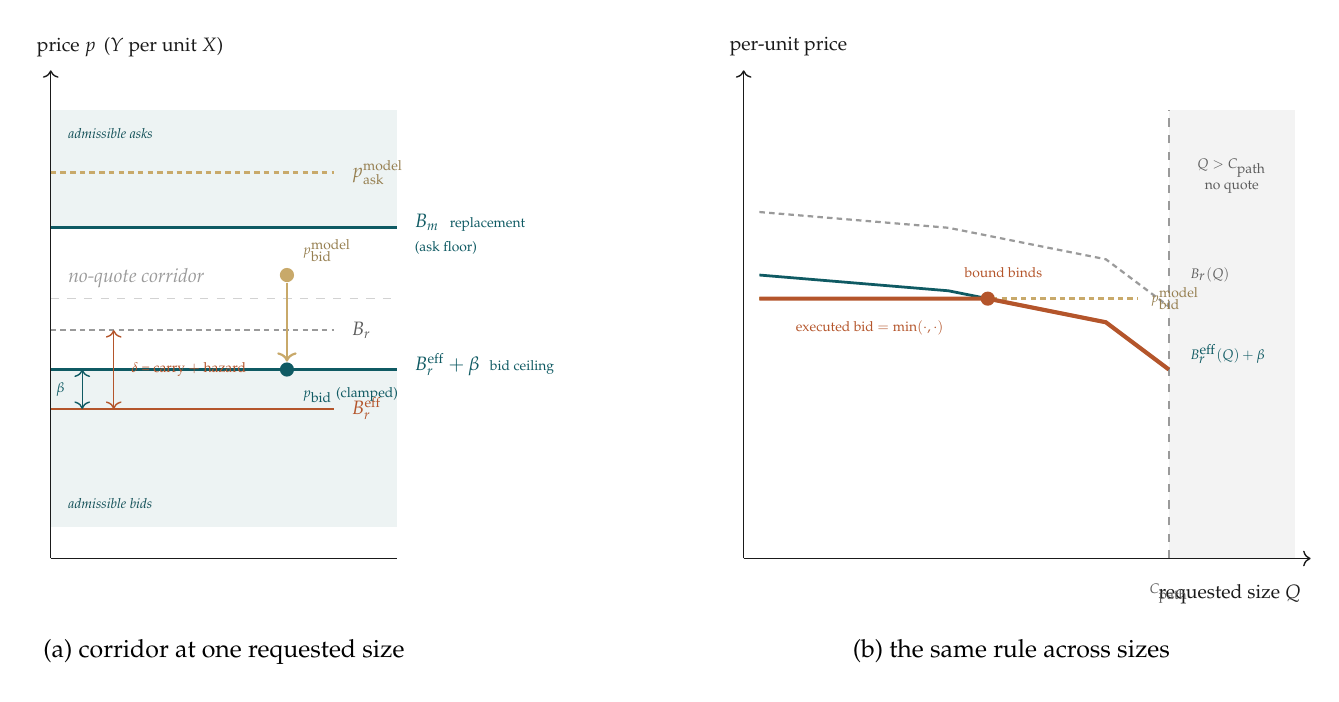
\begin{tikzpicture}[x=1mm,y=1mm,font=\scriptsize]

% ============ PANEL (a): corridor at a fixed size ============
\begin{scope}[shift={(0,0)}]
  \fill[tw-band] (8,42) rectangle (52,57);          % admissible asks
  \fill[tw-band] (8,4)  rectangle (52,24);          % admissible bids
  \draw[tw-grey!45,dashed,line width=0.3pt] (8,33) -- (52,33);
  \node[tw-grey,anchor=west] at (9,35.6) {\itshape no-quote corridor};

  \draw[->,tw-ink,line width=0.5pt] (8,0) -- (8,62);
  \node[tw-ink,anchor=west,font=\scriptsize] at (5,65) {price $p$\, ($Y$ per unit $X$)};
  \draw[tw-ink,line width=0.5pt] (8,0) -- (52,0);

  % ask side
  \draw[tw-teal,line width=1.1pt] (8,42) -- (52,42);
  \node[tw-teal,anchor=west,align=left] at (53,42.6) {$\Bm$ \;\tiny replacement};
  \node[tw-teal,anchor=west,font=\tiny] at (53,39.4) {(ask floor)};
  \draw[tw-sand,line width=0.9pt,dash pattern=on 2pt off 1.5pt] (8,49) -- (44,49);
  \node[tw-sand!75!black,anchor=west] at (45,49) {$p^{\mathrm{model}}_{\mathrm{ask}}$};
  \node[tw-teal!85!black,anchor=west,font=\itshape\tiny] at (9,54) {admissible asks};

  % bid side
  \draw[tw-grey,line width=0.7pt,dash pattern=on 2pt off 1.5pt] (8,29) -- (44,29);
  \node[tw-grey!60!black,anchor=west] at (45,29) {$\Br$};
  \draw[tw-teal,line width=1.1pt] (8,24) -- (52,24);
  \node[tw-teal,anchor=west,align=left] at (53,24.6) {$\Bre+\beta$ \;\tiny bid ceiling};
  \draw[tw-warn,line width=0.7pt] (8,19) -- (44,19);
  \node[tw-warn,anchor=west] at (45,19) {$\Bre$};
  \node[tw-teal!85!black,anchor=west,font=\itshape\tiny] at (9,7) {admissible bids};

  \draw[<->,tw-warn,line width=0.5pt] (16,29) -- (16,19);
  \node[tw-warn,anchor=west,font=\tiny,align=left] at (17,24) {$\delta$ = carry $+$ hazard};
  \draw[<->,tw-teal,line width=0.5pt] (12,19) -- (12,24);
  \node[tw-teal,anchor=east,font=\tiny] at (11,21.5) {$\beta$};

  \fill[tw-sand] (38,36) circle (0.9);
  \node[tw-sand!75!black,anchor=south west,font=\tiny] at (38.8,36.4) {$p^{\mathrm{model}}_{\mathrm{bid}}$};
  \draw[->,tw-sand,line width=0.8pt] (38,35) -- (38,25);
  \fill[tw-teal] (38,24) circle (0.9);
  \node[tw-teal,anchor=north west,font=\tiny] at (38.8,23) {$p_{\mathrm{bid}}$ (clamped)};

  \node[anchor=north,font=\small] at (30,-9) {(a) corridor at one requested size};
\end{scope}

% ============ PANEL (b): bounds as a function of size ============
\begin{scope}[shift={(90,0)}]
  \fill[tw-grey!12] (60,0) rectangle (76,57);
  \draw[tw-grey,dashed,line width=0.5pt] (60,0) -- (60,57);
  \node[tw-grey!60!black,anchor=north,align=center,font=\tiny] at (68,52)
       {$Q>C_{\mathrm{path}}$\\ no quote};

  \draw[->,tw-ink,line width=0.5pt] (6,0) -- (6,62);
  \node[tw-ink,anchor=west,font=\scriptsize] at (3,65) {per-unit price};
  \draw[->,tw-ink,line width=0.5pt] (6,0) -- (78,0);
  \node[tw-ink,anchor=north east,font=\scriptsize] at (78,-2) {requested size $Q$};
  \node[tw-grey!60!black,anchor=north,font=\tiny] at (60,-2) {$C_{\mathrm{path}}$};

  % nominal redemption bound
  \draw[tw-grey,line width=0.8pt,dash pattern=on 2pt off 1.5pt]
       (8,44) -- (32,42) -- (52,38) -- (60,32);
  \node[tw-grey!60!black,anchor=west,font=\tiny] at (61.5,36) {$\Br(Q)$};

  % delay-adjusted ceiling
  \draw[tw-teal,line width=1.0pt] (8,36) -- (32,34) -- (52,30) -- (60,24);
  \node[tw-teal,anchor=west,font=\tiny,align=left] at (61.5,26) {$\Bre(Q)+\beta$};

  % model bid
  \draw[tw-sand,line width=0.9pt,dash pattern=on 2pt off 1.5pt] (8,33) -- (56,33);
  \node[tw-sand!75!black,anchor=west,font=\tiny] at (56.5,33) {$p^{\mathrm{model}}_{\mathrm{bid}}$};

  % executed bid = min
  \draw[tw-warn,line width=1.5pt] (8,33) -- (37,33) -- (52,30) -- (60,24);
  \node[tw-warn,anchor=north,font=\tiny] at (22,31.4) {executed bid $=\min(\cdot,\cdot)$};
  \fill[tw-warn] (37,33) circle (0.9);
  \node[tw-warn,anchor=south,font=\tiny] at (39,34.4) {bound binds};

  \node[anchor=north,font=\small] at (40,-9) {(b) the same rule across sizes};
\end{scope}

\end{tikzpicture}
\caption{The quote corridor. \textbf{(a)} At one requested size, the inventory model chooses competitiveness
inside the shaded regions while the conversion bounds set the edges; an aggressive model bid is clamped
\emph{down} to $\Bre+\beta$, never up. Where the delay haircut $\delta$ exceeds the basis budget $\beta$, the
admissible ceiling sits strictly below the nominal bound $\Br$ --- the intended behaviour on a slow path.
\textbf{(b)} Across sizes, the bound is re-derived rather than extrapolated: the model price binds for small
requests, the conversion bound binds as fees, queue depth, and withdrawal liquidity degrade it, and beyond
$C_{\mathrm{path}}$ the adapter returns no bound and the strategy stops quoting rather than interpolating one.}
\label{fig:corridor}
\end{figure*}
% ------------------------------------------

\subsection{Replacement-bounded ask}

When a valid acquisition path exists, the maker's net ask is
\begin{equation}
  p_{\mathrm{ask}} \;=\; \max\!\big(p^{\mathrm{model}}_{\mathrm{ask}},\; \Bm(Q,S)\big).
\end{equation}
The maker may ask more, but not less, than the bounded cost of replacing the sold asset. Where no acquisition
bound exists, the ask is limited by available inventory and a separate exposure policy.

\subsection{Capacity, exposure, and the redemption pipeline}

A quotable size must satisfy all applicable limits:
\begin{multline*}
  Q \;\le\; \min\big(C_{\mathrm{path}},\, C_{\mathrm{strategy}},\, C_{\mathrm{portfolio}},\\
                     C_{\mathrm{queue}},\, C_{\mathrm{execution}}\big).
\end{multline*}
$C_{\mathrm{path}}$ is supplied by the adapter; $C_{\mathrm{strategy}}$ limits one order;
$C_{\mathrm{portfolio}}$ accounts for correlated strategies; and $C_{\mathrm{execution}}$ reflects balances,
allowance, and settlement constraints for the relevant side.

$C_{\mathrm{queue}}$ is specific to delayed paths and is the constraint most easily overlooked. Between fill and
settlement the maker holds a claim, not an asset. If $N$ is the notional already in flight and $N_{\max}$ the
configured pipeline limit, then $C_{\mathrm{queue}}$ must be sized so that $N + Q \le N_{\max}$. Without this
limit, a single stress episode can convert the entire wallet into unsettled claims at exactly the moment the
declared delay bound is least likely to hold.

Capacity is directional. A bid consumes $Y$ and acquires $X$; an ask consumes $X$ and acquires $Y$. Each fill
updates exposure in the direction implied by the acquired asset and releases exposure only when the configured
recycling or hedge action is \emph{observed to settle} --- not when it is submitted.

\subsection{Adverse selection and the freshness window}

The corridor bounds what the maker can lose relative to redemption; it does not assume the flow is random. It is
not. A maker quoting off a conversion bound is systematically the counterparty to holders who want immediacy, and
that demand is strongest precisely when the discount is widest and the queue is longest --- the two variables that
degrade the bound are positively correlated with arrival intensity.

Three distinct exposures follow, and they should not be conflated.

\textbf{Stale-state pick-off.} The bound is computed from state observed at $t$ and executed at $t' \le t+\tau$.
Any adverse movement of the conversion rate inside $\tau$ is capturable by a faster counterparty. Unlike a
constant-function market maker, whose loss-versus-rebalancing scales with the volatility of an external price the
pool does not observe, Tidewater's reference is on-chain state that it reads directly; the exposure is therefore
bounded by $\tau$ and by the adapter's declared state-movement bound, not by the arbitrageur's speed advantage
over an oracle. Shrinking $\tau$ shrinks this term monotonically, at the cost of quote availability.

\textbf{Basis drift.} Buying at $\Bre$ protects the maker against redemption value, not against the market. If the
discount widens after a fill, the maker has not lost against the redemption bound but has forgone a better entry.
$\beta$ is the budget for this and nothing else; it should be set from the observed distribution of discount
persistence, not from a desired fill rate.

\textbf{Queue extension.} The one exposure the corridor cannot bound. If realised $T$ exceeds $\bar{T}$, the
carry component of $\delta$ was undersized and Proposition~\ref{prop:delay} does not apply. This is why $\bar T$
must come from an adapter that models the queue, why $\lambda$ exists, and why $N_{\max}$ is a hard limit rather
than a soft target.

% =====================================================================
\section{Safety properties}

The following properties are conditional on correct adapter bounds, fee treatment, arithmetic, and execution of
the approved path.

\begin{proposition}[Per-fill redemption-relative loss, atomic paths]
\label{prop:atomic}
Suppose Tidewater buys $Q$ units of $X$ at maker-net price $p$, the bid rule enforces $p \le \Br(Q,S)+\beta$, the
path is atomic ($\bar T = 0$, $\lambda=0$), and redemption returns at least $\Lb(Q,S)$. Then the loss relative to
immediate redemption is at most $Q\beta$ units of $Y$.
\end{proposition}

\begin{proof}
The maker pays $Qp$. By the bid rule, $Qp \le Q(\Br+\beta) = \Lb(Q,S) + Q\beta$. Redemption returns at least
$\Lb(Q,S)$, so payment minus redemption output is at most $Q\beta$.
\end{proof}

\begin{proposition}[Carry-adjusted loss, delayed paths]
\label{prop:delay}
Suppose Tidewater buys $Q$ units of $X$ at maker-net price $p$ at time $t$, the bid rule enforces
$p \le \Bre(Q,S) + \beta$, settlement occurs at $t + T$ with $T \le \bar{T}(Q,S)$, and redemption returns at least
$\Lb(Q,S)$. Then, valuing proceeds at the maker's carry rate $r$, the present-value loss relative to redemption is
at most $Q(\beta - \lambda)$ units of $Y$, and is non-positive whenever $\lambda \ge \beta$.
\end{proposition}

\begin{proof}
The proceeds $\Lb(Q,S)$ arrive at $t+T$ and are worth at least $\Lb(Q,S)(1 - r\bar{T})$ at $t$, since
$T \le \bar T$ and $1/(1+r\bar T) \ge 1 - r\bar T$. Per unit this is $\Br(1-r\bar T) = \Br - \Br r \bar T$. By
definition $\Bre = \Br - \Br r\bar T - \lambda$, so the present value per unit is at least $\Bre + \lambda$. The
bid rule gives $p \le \Bre + \beta$. Subtracting, the per-unit present-value loss is at most
$(\Bre + \beta) - (\Bre + \lambda) = \beta - \lambda$. Multiplying by $Q$ gives the result.
\end{proof}

\begin{proposition}[Aggregate bounded basis budget]
For fills $i = 1,\dots,n$ that each satisfy Proposition~\ref{prop:atomic} or~\ref{prop:delay} and jointly remain
within their declared route, pipeline, and shared capacities, aggregate loss is at most $\sum_i Q_i \beta_i$.
\end{proposition}

\noindent This is an accounting bound, not a claim of statistical independence. Portfolio and pipeline capacity
must still constrain correlated fills whose redemption paths compete for the same liquidity or the same queue.

\begin{proposition}[Ask-side replacement protection]
Suppose the maker sells $Q$ units of $X$ at maker-net price $p$, the ask rule enforces $p \ge \Bm(Q,S)$, and the
approved path can acquire $Q$ units for at most $\Mb(Q,S)$. Then the sale proceeds are sufficient for the bounded
acquisition cost.
\end{proposition}

\begin{proof}
$Qp \ge Q\Bm = \Mb(Q,S)$.
\end{proof}

\begin{proposition}[Fee conservation]
For a gross fee amount $F$ with non-negative allocations $F_1,\dots,F_k$, the implementation must enforce
$\sum_j F_j = F$.
\end{proposition}

\noindent Integer remainders are assigned deterministically; they may not disappear or be minted through
independent rounding. Corridor checks use the maker-net cashflow after any fee charged to the maker.

\subsection*{Limits of the propositions}

These results do not guarantee a profit in a fiat numeraire and do not protect against loss after the reference
asset itself depegs. They do not cover an issuer default, governance seizure, permission revocation, invalid
adapter, chain failure, or a conversion transaction that cannot be executed under the adapter's assumptions.
Proposition~\ref{prop:delay} in particular fails if realised settlement time exceeds $\bar T$; a delay bound is an
assumption about the issuer's queue, and no arithmetic in this paper makes that assumption true.

% =====================================================================
\section{State and transition system}

For strategy $g$, define the safety-relevant state
\[
  \Sigma_g = (A_g, R_g, E_g, N_g, V_g, P_g, n_g, t_g),
\]
where $A_g$ is adapter state and version; $R_g$ is the immutable or versioned risk profile; $E_g$ is reserved and
realised portfolio exposure; $N_g$ is in-flight redemption notional; $V_g$ is the Aqua virtual-balance view; $P_g$
is the relevant physical balance and allowance view; $n_g$ is a configuration nonce; and $t_g$ is the state
observation time or block.

% ---------------- FIGURE 2 ----------------
\begin{figure*}[t]
\centering
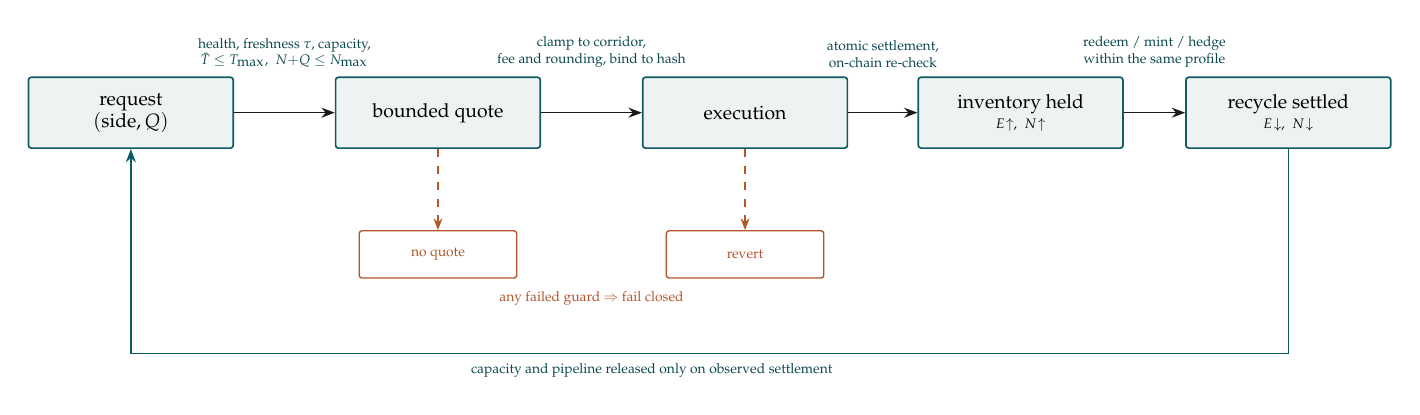
\begin{tikzpicture}[
  x=1mm,y=1mm,font=\scriptsize,
  box/.style={draw=tw-teal,line width=0.6pt,fill=tw-band,rounded corners=1pt,
              minimum width=26mm,minimum height=9mm,align=center,inner sep=2pt},
  fail/.style={draw=tw-warn,line width=0.5pt,fill=white,rounded corners=1pt,
               minimum width=20mm,minimum height=6mm,align=center,inner sep=2pt,
               text=tw-warn,font=\tiny},
  ar/.style={-{Stealth[length=1.7mm]},tw-ink,line width=0.55pt},
  fr/.style={-{Stealth[length=1.5mm]},tw-warn,line width=0.45pt,dashed}
]

\node[box] (req)   at (15,26)  {request\\$(\mathrm{side},Q)$};
\node[box] (quote) at (54,26)  {bounded quote};
\node[box] (exec)  at (93,26)  {execution};
\node[box] (hold)  at (128,26) {inventory held\\[-1pt]\tiny $E\!\uparrow$,\; $N\!\uparrow$};
\node[box] (rec)   at (162,26) {recycle settled\\[-1pt]\tiny $E\!\downarrow$,\; $N\!\downarrow$};

\draw[ar] (req)   -- (quote);
\draw[ar] (quote) -- (exec);
\draw[ar] (exec)  -- (hold);
\draw[ar] (hold)  -- (rec);

\node[anchor=south,align=center,font=\tiny,tw-teal!80!black] at (34.5,30.5)
     {health, freshness $\tau$, capacity,\\ $\bar T\le T_{\max}$,\; $N{+}Q\le N_{\max}$};
\node[anchor=south,align=center,font=\tiny,tw-teal!80!black] at (73.5,30.5)
     {clamp to corridor,\\ fee and rounding, bind to hash};
\node[anchor=south,align=center,font=\tiny,tw-teal!80!black] at (110.5,30.5)
     {atomic settlement,\\ on-chain re-check};
\node[anchor=south,align=center,font=\tiny,tw-teal!80!black] at (145,30.5)
     {redeem / mint / hedge\\ within the same profile};

\node[fail] (nq) at (54,8)  {no quote};
\node[fail] (rv) at (93,8)  {revert};
\draw[fr] (quote) -- (nq);
\draw[fr] (exec)  -- (rv);
\node[anchor=north,font=\tiny,tw-warn] at (73.5,4.5) {any failed guard $\Rightarrow$ fail closed};

\draw[ar,tw-teal] (rec.south) -- ++(0,-26)
      -- node[below,font=\tiny,tw-teal!80!black,pos=0.55]
         {capacity and pipeline released only on observed settlement}
      ($(req.south)+(0,-26)$) -- (req.south);

\end{tikzpicture}
\caption{The strategy transition system. Every forward edge is guarded and every guard fails closed. Exposure $E$
and in-flight pipeline notional $N$ are released only when recycling is observed to settle --- not when it is
submitted --- so a lengthening queue tightens quoting automatically instead of silently accumulating unsettled
claims.}
\label{fig:states}
\end{figure*}
% ------------------------------------------

\subsection{Quote transition}

For a request $(\text{side},Q)$, the quote transition:

\begin{enumerate}[label=\arabic*.]
  \item verifies adapter health, freshness against $\tau$, permissions, and path capacity;
  \item computes the maker-net conversion bound for $Q$, together with $\bar{T}$, and rejects the path if
        $\bar{T} > T_{\max}$;
  \item applies the delay haircut $\delta$ to obtain $\Bre$;
  \item checks strategy, portfolio, pipeline, virtual-balance, physical-balance, and allowance limits;
  \item applies the bid or ask clamp;
  \item converts the maker-net result into the displayed settlement amount, including fees and conservative
        rounding; and
  \item binds the quote to the program hash, risk-profile version, nonce, amount limit, delay bound, and deadline.
\end{enumerate}

No quote is returned when any required value is unavailable or internally inconsistent.

\subsection{Execution transition}

At execution, every mutable condition needed for safety must either be re-evaluated or bounded by a condition
encoded in the executable program. A stale off-chain quote is not a substitute for an on-chain check. On success,
settlement transfers the directional assets, accounts for the fee, and updates both exposure and pipeline
notional. On any failed assertion the whole operation reverts. Partial success is not a valid Tidewater
transition.

\subsection{Recycling transition}

A redemption, mint, or hedge transforms acquired inventory and releases exposure. A keeper may propose or submit
this transition, but correctness cannot depend on the keeper choosing a favourable price. The transaction must
remain within the same adapter and risk constraints or use a separately authorised execution policy. For delayed
paths the transition has two observable stages --- request and claim --- and pipeline notional is released only at
the second.

% =====================================================================
\section{Composition with Aqua and SwapVM}

\subsection{Aqua accounting}

Aqua records virtual balances by maker, application, strategy hash, and token while the physical tokens remain in
the maker's wallet. This allows the same physical wallet balance to support several strategies without depositing
assets into a separate pool.

Virtual allocation is not a guarantee that every correlated strategy can settle simultaneously. If several
strategies consume the same physical balance, a later fill can fail because the wallet balance or allowance is
insufficient. Tidewater therefore treats physical liquidity as a portfolio resource and applies an aggregate cap
in addition to Aqua's per-strategy virtual accounting.

\subsection{SwapVM execution}

The \texttt{AquaSwapVMRouter} is both the SwapVM execution entry point and the Aqua application used during
settlement. The \texttt{AquaAMM} template constructs programs and orders; it is not a second settlement
application.

Tidewater's corridor logic can be represented only through a reviewed composition whose quote-time and swap-time
behaviour are consistent. Where SwapVM's native instruction set cannot express an asset-specific check, the
computation is delegated to an \emph{extruction} --- an external, pinned contract invoked by the program to
perform that check and return a bounded value. An extruction is not a convenience: its exact bytecode,
dependencies, and pinned commit form part of the trusted computing base and are committed into strategy identity
alongside the program itself. Unsupported or non-deterministic instruction compositions are outside the mechanism
defined here.

\subsection{Strategy identity}

The executable program, adapter identifiers, extruction commits, risk-profile version, delay parameters, fee
configuration, and relevant token addresses are committed into the strategy identity. A material change produces a
new program or strategy hash. This prevents an order approved under one set of assumptions from silently
inheriting another.

% =====================================================================
\section{Adapter semantics}

An adapter is a conservative risk boundary, not a generic token-rate reader. For each direction it must expose:

\begin{itemize}[label=--]
  \item a bound and the amount over which it applies;
  \item path capacity and the reason for any tighter limit;
  \item a settlement delay bound $\bar T$ and the queue model that justifies it;
  \item state freshness and a version or digest;
  \item health, pause, and permission status;
  \item whether execution is atomic, delayed, or conditional; and
  \item the rounding and fee assumptions used in the bound.
\end{itemize}

Adapters fail closed. A revert, malformed return, stale state, unbounded settlement time, unsupported asset
behaviour, or loss of permission produces no bound. Shared libraries may normalise decimals and common vault
behaviour, but each supported asset requires a manifest and conformance tests against its actual contracts.

The normative interface and conformance requirements are defined in the separate \emph{Tidewater Asset Adapter
Standard}.

% =====================================================================
\section{Fees, arithmetic, and rounding}

Let the gross fee on a settlement amount be $F$. Fee recipients have allocation weights $\alpha_1,\dots,\alpha_k$
with $\alpha_j \ge 0$ and $\sum_j \alpha_j = 1$. The commercial choice of weights is external to this mechanism;
the technical requirements are conservation, deterministic rounding, and correct incidence.

The implementation uses fixed-point integer arithmetic with a declared scale $W$ (for example $W = 10^{18}$).
Prices are $W$-scaled ratios, and this has one consequence that must be stated explicitly because it is the
easiest place to lose the entire guarantee: a per-unit bound is never computed as an integer division of an amount
by an amount. The correct form is
\[
  \Br \;=\; \Big\lfloor \tfrac{\Lb \cdot W}{Q} \Big\rfloor, \qquad
  \Bm \;=\; \Big\lceil  \tfrac{\Mb \cdot W}{Q} \Big\rceil,
\]
evaluated with a full-width intermediate product. Computing $\Lb / Q$ first truncates to zero for any same-decimal
pair and silently produces a bound of zero or one.

The implementation must additionally:

\begin{itemize}[label=--]
  \item round redemption outputs and delay-adjusted bounds down;
  \item round acquisition costs and maker payments up where necessary for safety;
  \item round the delay haircut $\delta$ up, so that $\Bre$ is never overstated;
  \item calculate the gross fee once and split that integer amount;
  \item assign all division remainders by a declared rule;
  \item reject intermediate overflow and invalid decimal scaling; and
  \item apply corridor checks to maker-net amounts, not a pre-fee display price.
\end{itemize}

Exact-input and exact-output requests must converge on the same economic rule. An exact-output solver may use
bounded iteration, but the final executable amounts must independently satisfy capacity, exposure, pipeline, and
corridor checks.

% =====================================================================
\section{Maker economics}
\label{sec:econ}

The safety propositions bound loss. They say nothing about return, and a mechanism that only bounds loss is not
yet a business. This section states the return model explicitly so that its parameters can be argued with. All
figures below are illustrative arithmetic under stated assumptions, not measured results.

\subsection{Where the return comes from}

The maker's gross margin on a bid fill is the distance between what it pays and what the path returns:
$\Br - p$ per unit. Under Equation~\eqref{eq:bid} this is at least $-\beta$, and in practice it equals the
discount at which immediacy-seeking flow is willing to sell. Write $\bar{d}$ for the average captured discount per
unit of notional, net of the fee paid away and of gas, and $T_c$ for the full cycle time --- fill, redemption
request, settlement, redeployment. Let $\bar{u}$ be the time-averaged fraction of the maker's $Y$ balance
committed to the strategy.

The arbitrage component of annual return on the wallet balance is then
\begin{equation}
  \mathrm{APR}_{\mathrm{arb}} \;=\; \bar{u}\,\bar{d}\,\frac{365}{T_c},
  \label{eq:arb}
\end{equation}
with $T_c$ in days. Equation~\eqref{eq:arb} makes the two binding constraints legible, and they are not the ones
most quoting strategies optimise. Cycle time enters linearly: halving $T_c$ doubles the return from the same
discount, which is why $\bar T$ is an economic parameter and not only a safety one. Utilisation
$\bar u$ is the harder constraint --- in calm markets discounted flow is scarce, and a maker that widens $\beta$
to raise $\bar u$ is buying volume with the same budget that funds its loss bound.

\subsection{The shared-liquidity term}

For a dedicated-vault maker, the idle fraction $1 - \bar{u}$ is dead capital, recoverable only by bolting a
separate lending integration onto the vault and accepting the additional smart-contract surface that entails.
Under Aqua the physical balance never leaves the wallet, so it continues to serve any other strategy or yield
position authorised against it, except while a specific settlement is in flight. Writing $y_{\mathrm{base}}$ for
the return the same balance earns in its other roles and $\bar{n}$ for the time-averaged fraction sitting in an
unsettled redemption claim,
\begin{equation}
  \mathrm{APR}_{\mathrm{total}} \;=\; \bar{u}\,\bar{d}\,\frac{365}{T_c}
        \;+\; y_{\mathrm{base}}\,(1 - \bar{n}).
  \label{eq:total}
\end{equation}

The structural point is that $\bar{n} \ll 1 - \bar{u}$. Capital is genuinely unavailable only during settlement,
not during the far longer periods of simply standing ready to quote. A dedicated vault must reserve for the
\emph{option} to fill; a Tidewater strategy reserves only for fills that actually occurred. This is the mechanism
by which the same discount capture, on the same asset, at the same $\bar u$, produces a strictly higher return per
unit of committed capital --- and it is a property of the settlement layer, not of clever pricing.

\subsection{Sensitivity}

Table~\ref{tab:sens} evaluates Equation~\eqref{eq:arb} at $\bar{u} = 0.40$, holding the discount and cycle time as
free parameters. It excludes $y_{\mathrm{base}}$, which adds to every cell.

\begin{table}[h]
\centering\small
\caption{Illustrative $\mathrm{APR}_{\mathrm{arb}}$ at $\bar{u}=0.40$, per Equation~\eqref{eq:arb}. Rows are
average captured discount; columns are full cycle time in days.}
\label{tab:sens}
\begin{tabular}{@{}lccc@{}}
\toprule
& \multicolumn{3}{c}{cycle time $T_c$ (days)} \\
\cmidrule(l){2-4}
avg.\ discount $\bar{d}$ & 0.5 & 1.5 & 4.0 \\
\midrule
3 bps  & 8.8\%  & 2.9\% & 1.1\% \\
5 bps  & 14.6\% & 4.9\% & 1.8\% \\
10 bps & 29.2\% & 9.7\% & 3.7\% \\
\bottomrule
\end{tabular}
\end{table}

Two readings matter. First, the plausible operating region for a competitive maker on a liquid reference asset is
the middle of this table --- single-digit returns on committed capital, before $y_{\mathrm{base}}$ --- and any
projection materially outside it is asserting either an uncontested discount or a queue that does not exist.
Second, the ten-basis-point row is not a target to be reached by widening $\beta$. A larger $\beta$ raises
$\bar{u}$ and lowers realised $\bar{d}$ simultaneously, and Proposition~\ref{prop:delay} converts the difference
directly into bounded loss. The parameters that improve returns without spending the loss budget are $T_c$ and
$\bar{n}$, both of which are properties of the path and the settlement layer rather than of the quote.

% =====================================================================
\section{Security and trust assumptions}

Tidewater relies on the following components:

\begin{enumerate}[label=\arabic*.]
  \item the settlement chain and token contracts behave according to their specified interfaces;
  \item Aqua and the selected SwapVM execution path correctly account and settle transfers;
  \item each adapter's output and delay bounds are conservative for its declared state transitions;
  \item risk-profile authorisation and strategy identity cannot be bypassed;
  \item fee-on-transfer, rebasing, callback, permissioned, and non-standard token behaviour is either modelled or
        rejected; and
  \item aggregate exposure and pipeline notional are not understated across strategies sharing physical liquidity
        or a conversion path.
\end{enumerate}

Important failure modes include rate manipulation, preview/execution divergence, capacity exhaustion between quote
and fill, queue extension after a request is submitted, stale permissions, reentrancy, rounding inversion,
fixed-point scale confusion, malicious token callbacks, strategy-hash confusion, replay of old configurations, and
correlated balance depletion. The system must revert on uncertainty rather than substitute an optimistic value.

The mechanism deliberately distinguishes a safety monitor from a trusted price oracle. Monitoring and keepers may
improve availability and recycling speed, but an unavailable keeper should reduce or stop quoting rather than
invalidate the bound.

% =====================================================================
\section{Generalisation}

The construction applies whenever an asset regime can supply conservative conversion bounds, capacities, delay
bounds, and state-transition assumptions. Immediate vault redemption is the regime with $\bar T = 0$. Queued
staking exits require a delay and slash model and are the regime for which Section~\ref{sec:delay} exists.
Permissioned tokenised assets require transfer eligibility, market-calendar, and settlement state. Wrapped assets
require bridge or custodian assumptions.

These regimes should not be hidden behind one permissive adapter. Each materially different regime is expressed
through a versioned adapter class and, where execution semantics differ, a versioned SwapVM program with its own
threat model. The reusable object is the bounded-quote framework, not an assertion that all redeemable assets are
equivalent.

% =====================================================================
\section{Conclusion}

Tidewater converts an asset-specific redemption property into an executable market-making constraint. Its bid and
ask rules separate competitiveness from safety: inventory logic selects a model quote, while conservative,
size-aware, delay-adjusted conversion bounds constrain the maker's net cashflow. Aqua supplies shared wallet
liquidity and settlement accounting; SwapVM supplies programmable execution; Tidewater supplies the adapter
semantics, portfolio and pipeline limits, quote clamps, and state checks needed to make the bound meaningful.

The resulting guarantee is intentionally narrow. Within a valid conversion path, its declared capacity, and its
declared settlement delay, the maker's carry-adjusted loss relative to redemption is bounded by an explicit
budget. Outside those assumptions, the mechanism fails closed rather than treating a nominal exchange rate as
executable value. The return model in Section~\ref{sec:econ} is stated with the same intent: the numbers that
matter are cycle time and the fraction of capital genuinely committed, and both are properties of the settlement
architecture rather than of the quote.

% =====================================================================
\appendix
\section*{Appendix A --- Reference quote algorithm}
\addcontentsline{toc}{section}{Appendix A}

\vspace{-2pt}
{\scriptsize
\begin{verbatim}
// All prices are W-scaled fixed point (W = 1e18).
// mulDivDown / mulDivUp use a full-width
// intermediate product; never divide amounts
// by amounts to obtain a price.

quote(request, state):
  require request.amount > 0
  require request.deadline >= now

  profile = loadRiskProfile(request.strategyId)
  require profile.active
  require request.programHash  == profile.programHash
  require request.configNonce  == profile.configNonce

  a = adapter.bound(request.base, request.quote,
                    request.side, request.amount,
                    state)

  require a.healthy
  require a.fresh              // age <= profile.tau
  require request.amount <= a.capacity
  require a.maxDelay <= profile.maxDelay

  require withinStrategyLimit(request, profile)
  require withinPortfolioLimit(request,
              state.exposure, profile)
  require withinPipelineLimit(request,
              state.inFlight, profile)
  require settlementLiquidityAvailable(request,
              state)

  model = inventoryModel(request, state, profile)

  if request.side == BID:
    // per-unit bound: scale first, then divide
    bound = mulDivDown(a.redeemLower, W,
                       request.amount)

    // delay haircut, rounded UP so that the
    // effective bound is never overstated
    carry = mulDivUp(bound,
              profile.carryRate * a.maxDelay,
              W * YEAR)
    delta = carry + profile.hazardHaircut
    effBound = (bound > delta) ? bound - delta : 0

    makerNet = min(model.bid,
                   effBound + profile.basisBudget)
  else:
    require a.hasAcquisitionBound
    bound = mulDivUp(a.acquireUpper, W,
                     request.amount)
    makerNet = max(model.ask, bound)

  settlement = addFeeAndRoundAgainstMaker(makerNet,
                   request)
  require recheckNetCorridor(settlement, a, profile)

  return bindToState(settlement, a, profile,
                     a.maxDelay, request.deadline)
\end{verbatim}
}

\section*{Appendix B --- Illustrative calculation}
\addcontentsline{toc}{section}{Appendix B}

\textbf{Atomic path.} Assume 100 $X$ can be redeemed in the same transaction for at least 99.70 $Y$ after all
modelled conversion costs. Then $\Br = 0.9970$ and $\bar T = 0$. If the inventory model would bid 1.0010 and
$\beta = 0$, Tidewater bids at most 0.9970. If $\beta = 0.0010$, it may bid at most 0.9980, and
Proposition~\ref{prop:atomic} limits redemption-relative loss to $100 \times 0.0010 = 0.10$ $Y$ on the fill.

\medskip
\noindent\textbf{Delayed path.} Take the same redemption bound, but through a withdrawal queue with
$\bar{T} = 2$ days, a maker carry rate of $r = 4\%$ per annum, and a hazard allowance
$\lambda = 0.0001$ $Y$ per unit. The carry component is
\[
  \Br\, r\, \bar T = 0.9970 \times 0.04 \times \tfrac{2}{365} \approx 0.000219,
\]
so $\delta \approx 0.000319$ and, rounding the haircut up, $\Bre = 0.99668$.

With $\beta = 0$ the bid ceiling is 0.99668 --- meaningfully below the 0.99700 that a delay-blind implementation
would have quoted, and that difference is precisely the compensation for two days of committed capital plus the
hazard allowance. With $\beta = 0.0010$ the ceiling is 0.99768, and Proposition~\ref{prop:delay} bounds the
present-value loss to $100 \times (0.0010 - 0.0001) = 0.09$ $Y$.

If the model would bid only 0.9940, the final bid is 0.9940; the corridor is a ceiling, not a requirement to quote
at it.

\medskip
\noindent\textbf{Ask side.} If acquiring 100 $X$ costs at most 100.40 $Y$, then $\Bm = 1.0040$, and an otherwise
lower model ask is raised to 1.0040 before fees are mapped to displayed settlement amounts.

% =====================================================================
\section*{References}

\begin{enumerate}[label={[\arabic*]}]
  \item 1inch Network. \emph{Aqua White Paper}.
  \item Ethereum Improvement Proposals. \emph{EIP-4626: Tokenized Vaults}.
  \item 1inch Network. \emph{SwapVM and SwapVM Template}.
  \item D. Niemerg, A. Robinson, and G. Roberts. \emph{YieldSpace: An Automated Liquidity Provider for Fixed
        Yield Tokens}.
\end{enumerate}

\end{document}
